%%%%%%%%%%%%%%%%%%%%%%%%%%%%%%%%%%%%%%%%%%%%%%%%%%%%%%%%%%%%%%%%%
% MUW Presentation
% LaTeX Template
% Version 1.0 (27/12/2016)
%
% License:
% CC BY-NC-SA 4.0 (http://creativecommons.org/licenses/by-nc-sa/3.0/)
%
% Created by:
% Nicolas Ballarini, CeMSIIS, Medical University of Vienna
% nicoballarini@gmail.com
% http://statistics.msi.meduniwien.ac.at/
%
% Customized for UAH by:
% David F. Barrero, Departamento de Automática, UAH
%%%%%%%%%%%%%%%%%%%%%%%%%%%%%%%%%%%%%%%%%%%%%%%%%%%%%%%%%%%%%%%%%

\documentclass[10pt,compress]{beamer} % Change 10pt to make fonts of a different size
\mode<presentation>

\usepackage[spanish]{babel}
\usepackage{fontspec}
\usepackage{tikz}
\usepackage{etoolbox}
\usepackage{xcolor}
\usepackage{xstring}
\usepackage{listings}

% Para el diagrama del controlador y robot, no reutilizable
\usepackage{tikz}
\usetikzlibrary{arrows,positioning,patterns} 
\tikzset{
    %Define standard arrow tip
    >=stealth',
    %Define style for boxes
    punkt/.style={
        rectangle,
        rounded corners,
        draw, very thick,
        text width=6.5em,
        minimum height=2em,
        text centered},
    % Define arrow style
	pil/.style={ 
		->, 
		thick, 
		shorten <=2pt, 
		shorten >=2pt,} 
} 

% Variables para el robot, no reutilizable
\newcommand{\nvar}[2]{%
    \newlength{#1}
	\setlength{#1}{#2}
}

% Define a few constants for drawing
\nvar{\dg}{0.3cm}
\def\dw{0.25}\def\dh{0.5}
\nvar{\ddx}{1.5cm}

% Define commands for links, joints and such
\def\link{\draw [double distance=1.5mm, very thick] (0,0)--}
\def\joint{%
    \filldraw [fill=white] (0,0) circle (5pt);
    \fill[black] circle (2pt);
}
\def\grip{%
    \draw[ultra thick](0cm,\dg)--(0cm,-\dg);
    \fill (0cm, 0.5\dg)+(0cm,1.5pt) -- +(0.6\dg,0cm) -- +(0pt,-1.5pt);
    \fill (0cm, -0.5\dg)+(0cm,1.5pt) -- +(0.6\dg,0cm) -- +(0pt,-1.5pt);
}
\def\robotbase{%
    \draw[rounded corners=8pt] (-\dw,-\dh)-- (-\dw, 0) --
       (0,\dh)--(\dw,0)--(\dw,-\dh);
    \draw (-0.5,-\dh)-- (0.5,-\dh);
    \fill[pattern=north east lines] (-0.5,-1) rectangle (0.5,-\dh);
}

% Draw an angle annotation
% Input:
%   #1 Angle
%   #2 Label
% Example:
%   \angann{30}{$\theta_1$}
\newcommand{\angann}[2]{%
    \begin{scope}[red]
    \draw [dashed, red] (0,0) -- (1.2\ddx,0pt);
    \draw [->, shorten >=3.5pt] (\ddx,0pt) arc (0:#1:\ddx);
    % Unfortunately automatic node placement on an arc is not supported yet.
    % We therefore have to compute an appropriate coordinate ourselves.
    \node at (#1/2-2:\ddx+8pt) {#2};
    \end{scope}
}

% Draw line annotation
% Input:
%   #1 Line offset (optional)
%   #2 Line angle
%   #3 Line length
%   #5 Line label
% Example:
%   \lineann[1]{30}{2}{$L_1$}
\newcommand{\lineann}[4][0.5]{%
    \begin{scope}[rotate=#2, blue,inner sep=2pt]
    \draw[dashed, blue!40] (0,0) -- +(0,#1)
  	  node [coordinate, near end] (a) {};
	\draw[dashed, blue!40] (#3,0) -- +(0,#1)
	  node [coordinate, near end] (b) {};
	\draw[|<->|] (a) -- node[fill=white] {#4} (b);
	\end{scope}
}

% Define the kinematic parameters of the three link manipulator.
\def\thetaone{30}
\def\Lone{2}
\def\thetatwo{30}
\def\Ltwo{2}
\def\thetathree{30}
\def\Lthree{1}

% Especial para estas diapositivas \usepackage[official]{eurosym}

\definecolor{dkgreen}{rgb}{0,0.6,0}
\definecolor{gray}{rgb}{0.5,0.5,0.5}
\definecolor{mauve}{rgb}{0.58,0,0.82}
 


\usetheme{UAH}
\usecolortheme{UAH}
\setbeamertemplate{navigation symbols}{} 
\setbeamertemplate{caption}[numbered]

%%%%%%%%%%%%%%%%%%%%%%%%%%%%%%%%%%%%%%%%%%%%%%%%%%%%%%%%%%%%%%%%%
%% Presentation Info
\title[Introduction to Robotics]{Introduction to Robotics}
\author{}
\institute{\asignatura}
\date{}
%%%%%%%%%%%%%%%%%%%%%%%%%%%%%%%%%%%%%%%%%%%%%%%%%%%%%%%%%%%%%%%%%


%%%%%%%%%%%%%%%%%%%%%%%%%%%%%%%%%%%%%%%%%%%%%%%%%%%%%%%%%%%%%%%%%
%% Descomentar para habilitar barra de navegación superior
\ponerNavegacion
%%%%%%%%%%%%%%%%%%%%%%%%%%%%%%%%%%%%%%%%%%%%%%%%%%%%%%%%%%%%%%%%%

%%%%%%%%%%%%%%%%%%%%%%%%%%%%%%%%%%%%%%%%%%%%%%%%%%%%%%%%%%%%%%%%%
%% Configuración de logotipos en portada
%% Opacidad de los logotipos
\newcommand{\opacidad}{1}
%% Descomentar para habilitar logotipo en pié de página de portada
\renewcommand{\logoUno}{Images/isg.png}
%% Descomentar para habilitar logotipo en pié de página de portada
%\renewcommand{\logoDos}{Images/CCLogo.png}
%% Descomentar para habilitar logotipo en pié de página de portada
%\renewcommand{\logoTres}{Images/ALogo.png}
%% Descomentar para habilitar logotipo en pié de página de portada
%\renewcommand{\logoCuatro}{Images/ELogo.png}
%%%%%%%%%%%%%%%%%%%%%%%%%%%%%%%%%%%%%%%%%%%%%%%%%%%%%%%%%%%%%%%%%

%%%%%%%%%%%%%%%%%%%%%%%%%%%%%%%%%%%%%%%%%%%%%%%%%%%%%%%%%%%%%%%%%
%% FOOTLINE
%% Comment/Uncomment the following blocks to modify the footline
%% content in the body slides. 


%% Option A: Title and institute
\footlineA
%% Option B: Author and institute
%\footlineB
%% Option C: Title, Author and institute
%\footlineC
%%%%%%%%%%%%%%%%%%%%%%%%%%%%%%%%%%%%%%%%%%%%%%%%%%%%%%%%%%%%%%%%%

\begin{document}

%%%%%%%%%%%%%%%%%%%%%%%%%%%%%%%%%%%%%%%%%%%%%%%%%%%%%%%%%%%%%%%%%
% Use this block for a blue title slide with modified footline
{\titlepageBlue
    \setbeamertemplate{headline}{}
	\setbeamercolor{frametitle}{bg=black}
	\setbeamercolor{normal text}{bg=black}
    \begin{frame}
        \titlepage
    \end{frame}
}

\begin{frame}[plain]{}
   \begin{block}{Objectives}
       \begin{itemize}
        \item Introduce main topics on Robotics
       \end{itemize}
   \end{block}

   \begin{block}{Bibliography}
       No suiteable bibliography
   \end{block}
\end{frame}

{
\eliminarNavegacion
\begin{frame}[shrink]{Table of Contents}
 \frametitle{Table of Contents}
 \tableofcontents
  % You might wish to add the option [pausesections]
\end{frame}
}

\section{Introduction}

\subsection{Introduction to robotics}
\begin{frame}{Introduction}{Introduction to Robotics (I)}
    \begin{columns}
 	   \column{.60\textwidth}
	   \begin{block}{Robot definition}
	   \begin{quote}
	   \textbf{Active}, \textbf{artificial agent} whose environment is the \textbf{physical
	   world} 
	   \end{quote}
	   \begin{flushright}
	   	\textit{Russell and Norvig}
		\end{flushright}
	   \end{block}
		\begin{itemize}
			\item Active: It is not a rock
			\item Artificial: It is not an animal
			\item Physical world: It is not just software
		\end{itemize}
 	   \column{.40\textwidth}
			\centering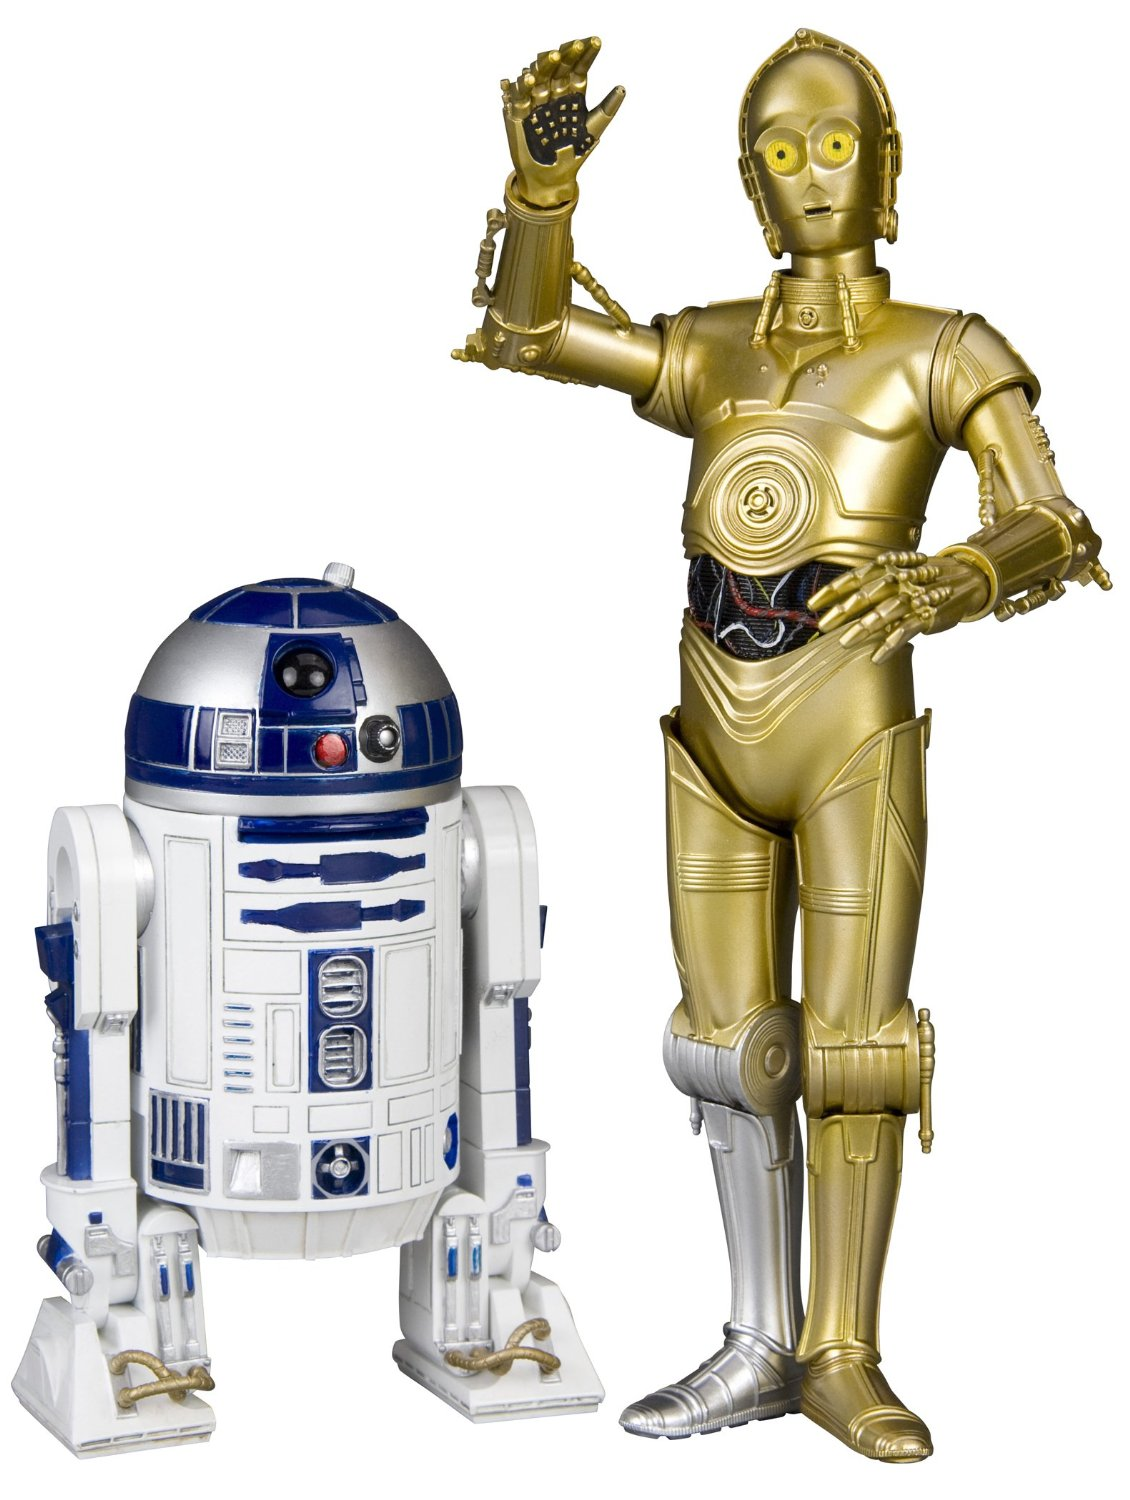
\includegraphics[width=0.8\linewidth]{figs/c3po.jpg}
	\end{columns}
\end{frame}

\begin{frame}{Introduction}{Introduction to Robotics (II)}
	Robotics also includes
	\begin{itemize}
		\item Robotic swarms \href{https://www.youtube.com/watch?v=xK54Bu9HFRw}{(Video)}
		\item Human-robot interfaces \href{https://www.youtube.com/watch?v=Qpn591m6hzU}{(Video)}, human-machine interfaces \href{https://www.youtube.com/watch?v=LJ0sIHj-OWo}{(Video)}, ...
	\end{itemize}

	Fields related to Robotics
	\begin{itemize}
		\item Mechanical engineering
		\item Electronics
		\item Artificial vision \href{https://www.youtube.com/watch?v=4KlYdCBdjEg}{(Video)}
		\item Machine Learning \href{https://www.youtube.com/watch?v=pgaEE27nsQw}{(Video)}
		\item Learning \href{https://www.youtube.com/watch?v=W\_gxLKSsSIE}{(Video)}
		\item Neural Networks \href{https://www.youtube.com/watch?v=xcIBoPuNIiw}{(Video)}
		\item Evolutionary Computation \href{https://www.youtube.com/watch?v=HgWQ-gPIvt4}{(Video)}
	\end{itemize}
\end{frame}

\begin{frame}{Introduction}{Introduction to Robotics (III)}
	Robots may be \alert{autonomous} or \alert{teleoperated}
	\begin{itemize}
		\item Greyscale between them
		\item We are interested in autonomous robots
	\end{itemize}
	Real-world is demanding
	\begin{itemize}
		\item \textbf{Inacessible}, the world is incompletely perceived by sensors
		\item \textbf{Non-deterministic}, the robot must deal with uncertainty
		\item \textbf{Non-episodic}, the effects of an action change over time
		\item \textbf{Dynamic}, the robot may need to deliberate or to act
		\item \textbf{Continous}, enumerating all the potential actions is inviable
	\end{itemize}
\end{frame}

\subsection{Applications}
\begin{frame}{Introduction}{Applications}
	\begin{itemize}
		\item Manufacturing and materials handling
		\item Survillance robots
		\item Hazardous environments
		\item Telepresence and virtual reality
		\item Augmentation of human abilities
		\item Prosthesis
		\item Space exploration
		\item Autonomous cars
		\item Security and defense
	\end{itemize}
\end{frame}

\subsection{Robot categories}
\begin{frame}{Introduction}{Robot categories}
	Three big categories
	\begin{itemize}
		\item \textbf{Manipulators}
		\item \textbf{Mobile robots}
		\item \textbf{Humanoids}
	\end{itemize}
	This classification is not strict
\end{frame}

\begin{frame}{Introduction}{Robot categories: Manipulators}
   \begin{columns}
 	   \column{.50\textwidth}
	   \begin{block}{Applications}
	   \begin{itemize}
	   \item Manufacturing
	   \item Robotically-assisted surgery 
	   \item Space
	   \item Harzadous materials
	   \end{itemize}
	   \end{block}
	   \href{https://www.youtube.com/watch?v=7coUcEHxnYA}{(Video robotic arm)}\\
	   \href{https://www.youtube.com/watch?v=sjAZGUcjrP8}{(Video production line)}


 	   \column{.50\textwidth}
			\centering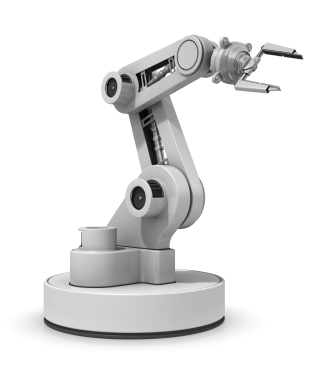
\includegraphics[width=0.5\linewidth]{figs/arm.jpeg}
			\centering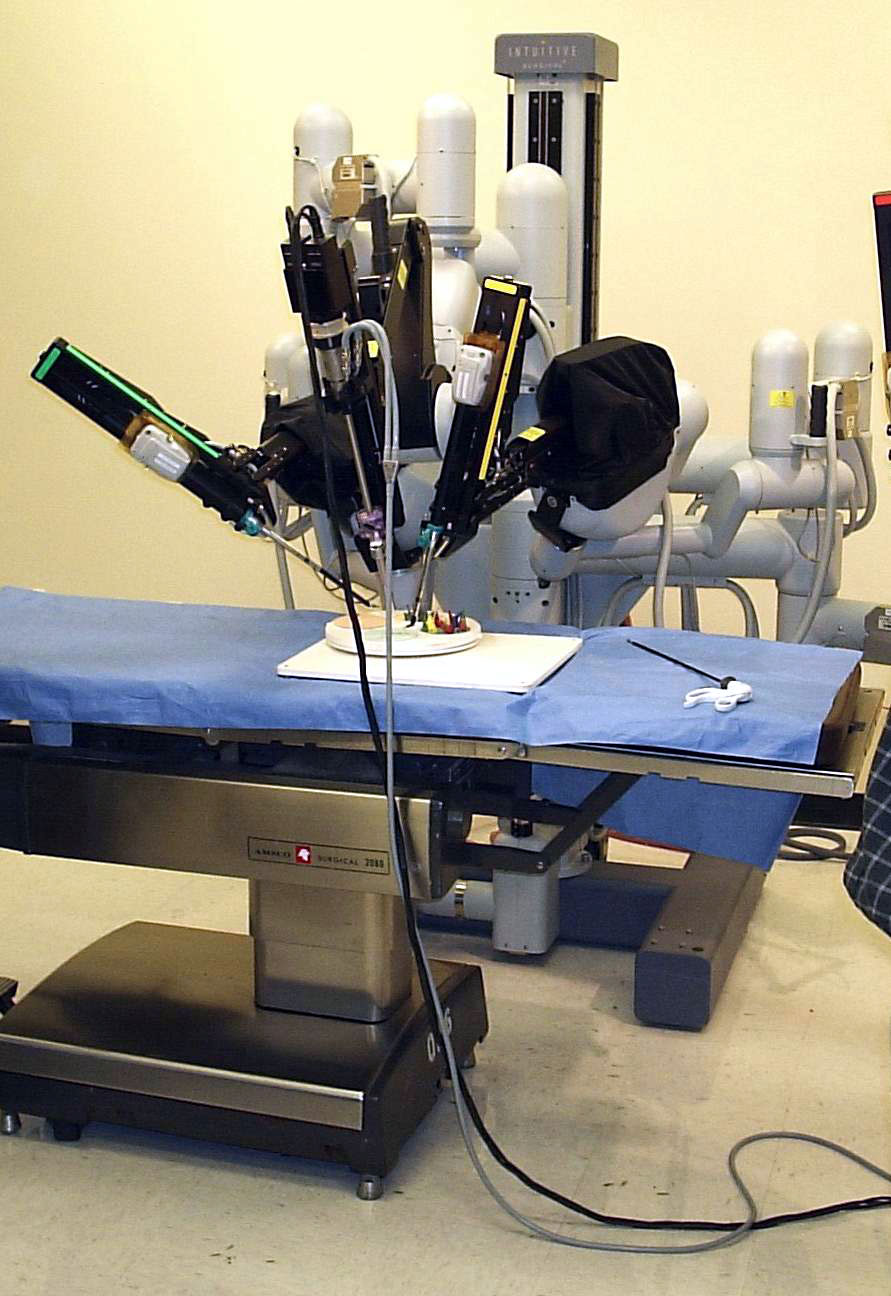
\includegraphics[width=0.5\linewidth]{figs/surgery.jpg}\\
			\centering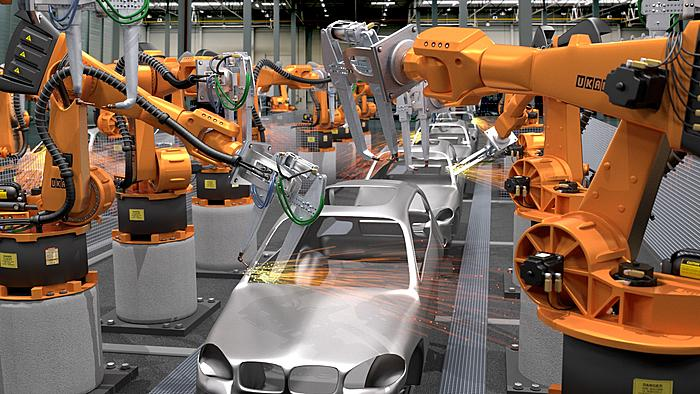
\includegraphics[width=0.5\linewidth]{figs/industrial.jpg}
			\centering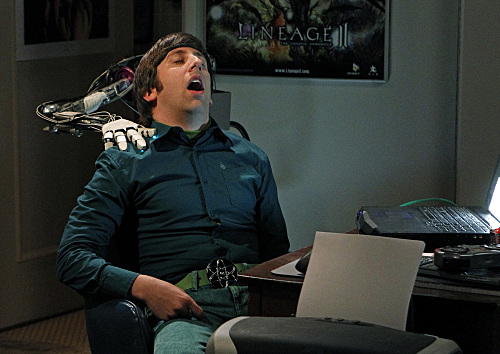
\includegraphics[width=0.5\linewidth]{figs/bigbangtheory.jpg}
	\end{columns}
\end{frame}

\begin{frame}{Introduction}{Robot categories: Mobile robots}
   \begin{columns}
 	   \column{.50\textwidth}
	   \begin{block}{Applications}
	   \begin{itemize}
	   \item Exploration
	   \item Harzadous environments
	   \item Defense and security
	   \item Surveillance
	   \item Telecare
	   \end{itemize}
	   Types: UAVs, UGVs, AUV, quads
	   \end{block}

	   \href{https://www.youtube.com/watch?v=oO\_Ohp1pHBw}{(Video UAV)}\\
	   \href{https://www.youtube.com/watch?v=ScTxzbZswdE}{(Video AUV)}\\
	   \href{https://www.youtube.com/watch?v=scc9cbsBKgM}{(Video Fukushima)}
	   
 	   \column{.50\textwidth}
			\centering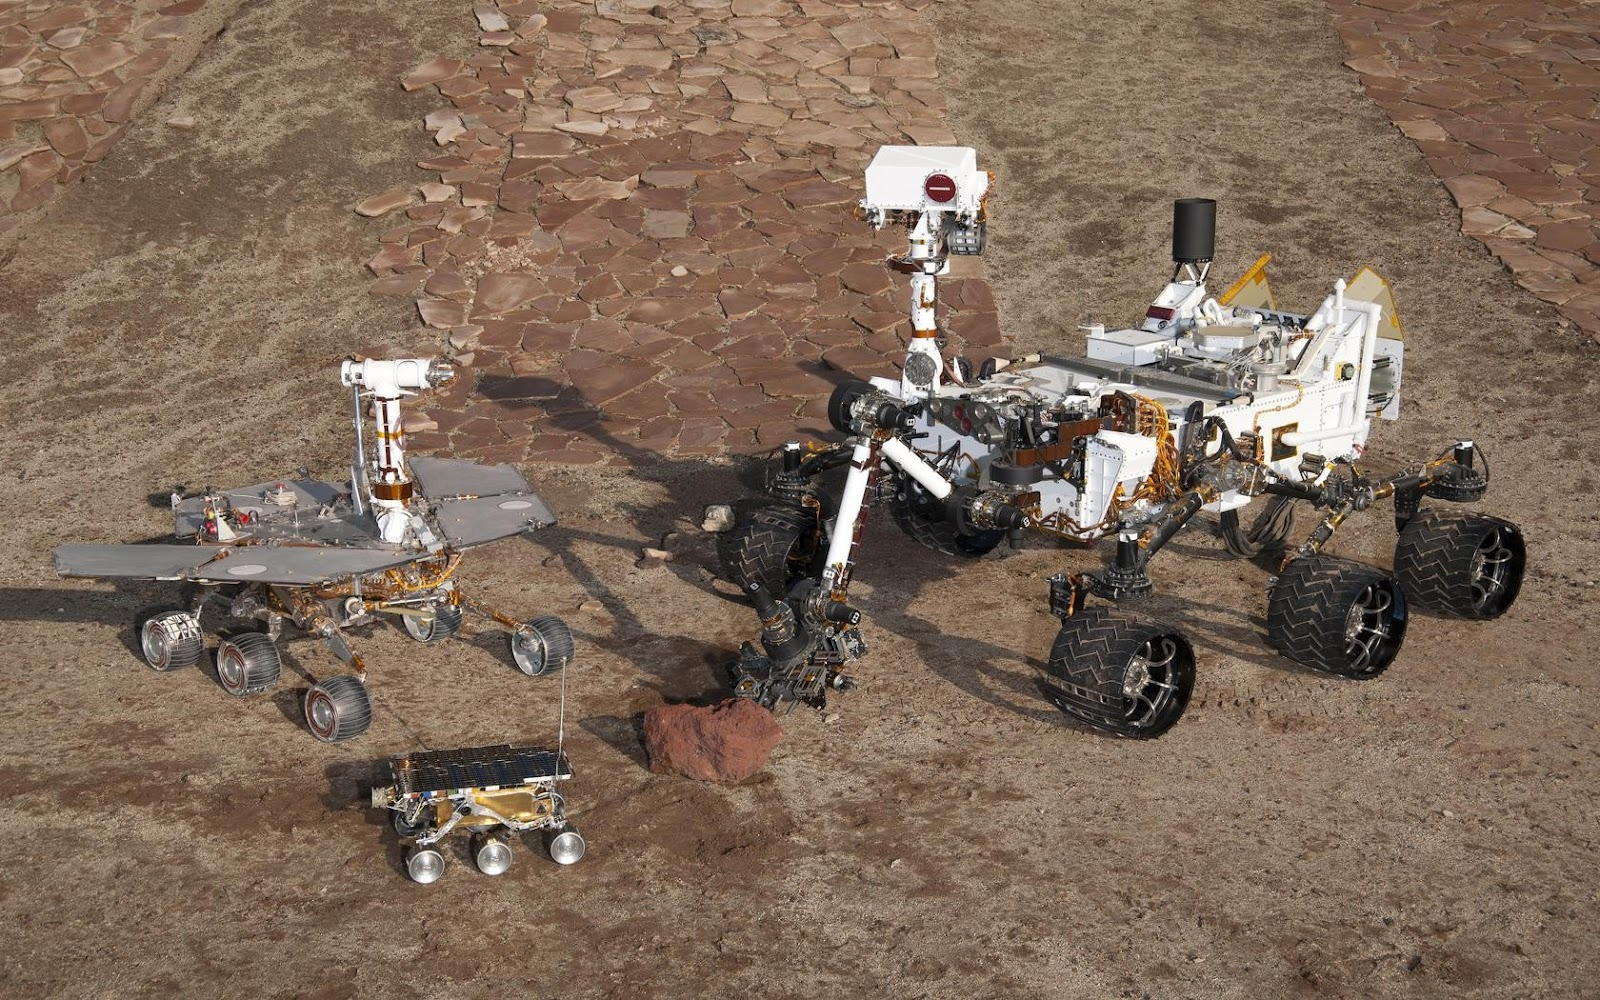
\includegraphics[width=0.5\linewidth]{figs/curiosity.jpeg}
			\centering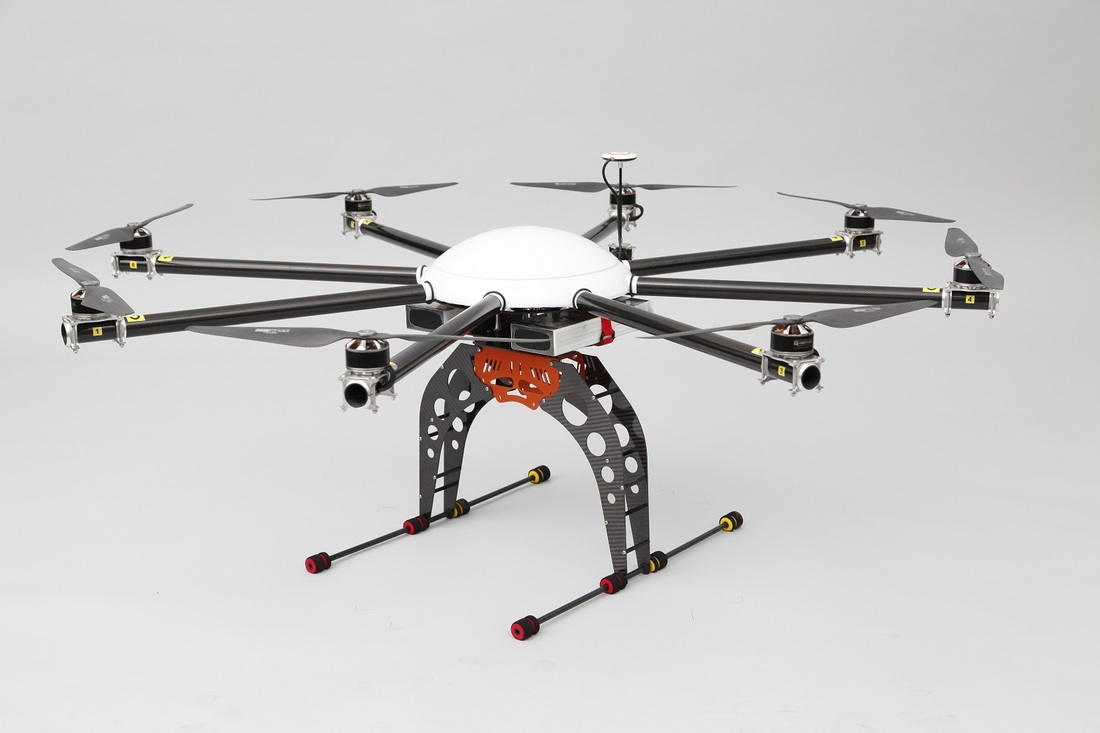
\includegraphics[width=0.5\linewidth]{figs/drone.jpg}\\
			\centering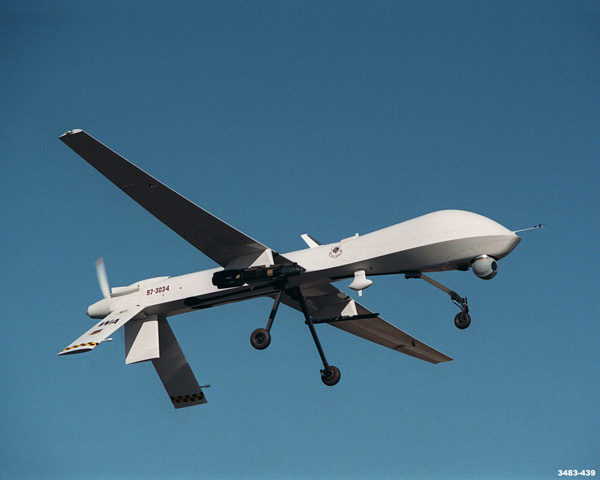
\includegraphics[width=0.5\linewidth]{figs/uav.jpg}
			\centering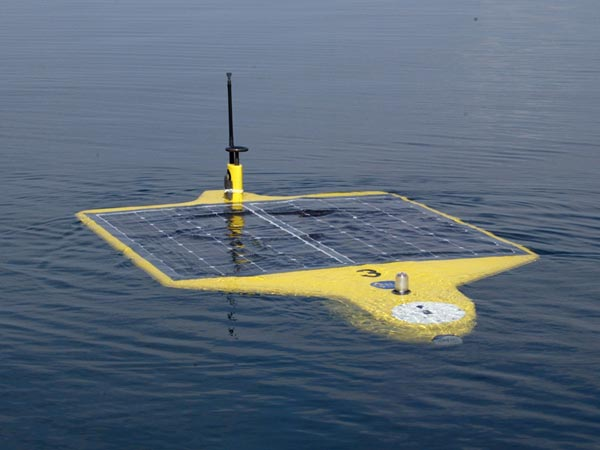
\includegraphics[width=0.5\linewidth]{figs/auv.jpg}
	\end{columns}
\end{frame}

\begin{frame}{Introduction}{Robot categories: Humanoids}
   \begin{columns}
 	   \column{.50\textwidth}
	   \begin{block}{Applications}
	   \begin{itemize}
	   \item Research
	   \item Enterteinment
	   \item Telecare
	   \end{itemize}
	   \end{block}

	   \href{https://www.youtube.com/watch?v=qsRsrMQy64k}{(Video Nao)}
	   \href{https://www.youtube.com/watch?v=M7nLQpWiy1o}{(Video Atlas)}
	   \href{https://www.youtube.com/watch?v=BGOUSvaQcBs}{(Video DARPA)}
	   \href{https://www.youtube.com/watch?v=7A_QPGcjrh0}{(Video DARPA bonus track)}

 	   \column{.50\textwidth}
			\centering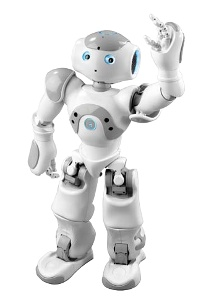
\includegraphics[width=0.4\linewidth]{figs/nao.jpg}
			\centering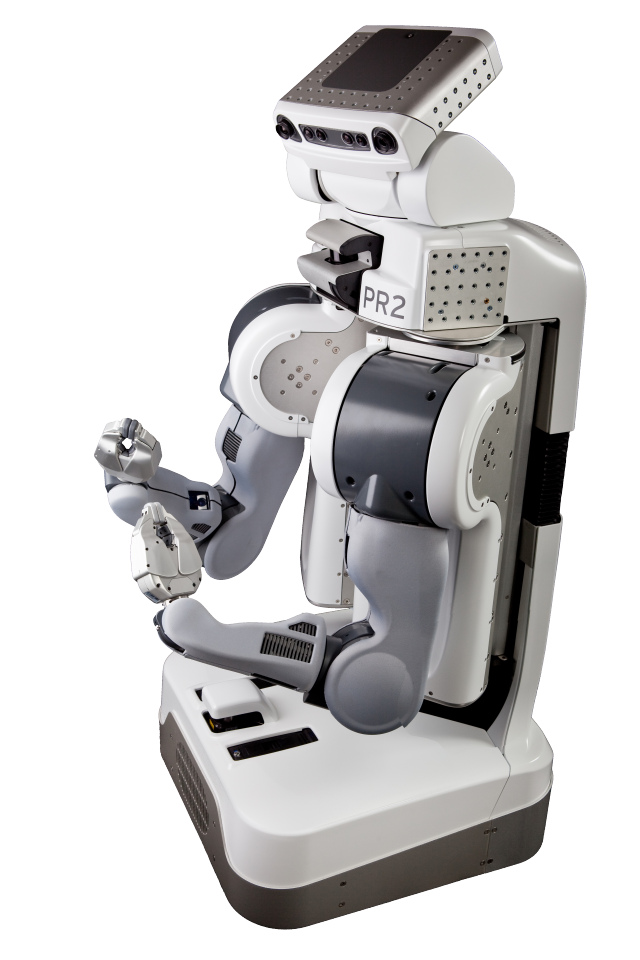
\includegraphics[width=0.4\linewidth]{figs/pr2.jpg}\\
			\centering
\includegraphics[width=0.4\linewidth]{figs/bender.png}
			\centering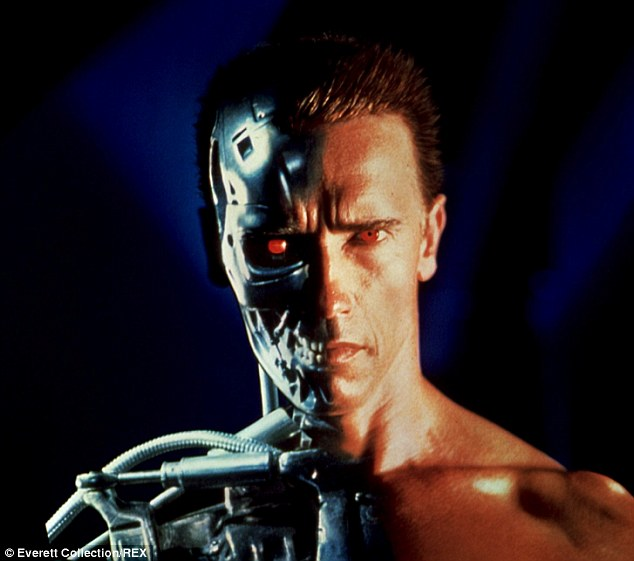
\includegraphics[width=0.4\linewidth]{figs/terminator.jpg}
	\end{columns}
\end{frame}


\subsection{Components}
\begin{frame}{Introduction}{Components}
	Any robot contains three components
	\begin{itemize}
		\item \textbf{Effectors} (actuator). Affects the environment
		\item \textbf{Sensors}. Provides knowledge about the environment
		\item \textbf{Controller}. Takes decisions
	\end{itemize}

	\begin{center}
		\begin{tikzpicture}[node distance=1cm, auto,]
		 %nodes
		  \node[punkt] (controller) {Controller};
			 % We make a dummy figure to make everything look nice.
		  \node[above=of controller] (dummy) {};
		  \node[right=of dummy] (t) {Effectors}
			      edge[pil,<-,bend left=45] (controller.east); % edges are used to connect two nodes
		  \node[left=of dummy] (g) {Sensors}
		      edge[pil,->,bend right=45] (controller.west)
			  edge[pil,<-, bend left=45] node[auto] {Environment} (t);
		\end{tikzpicture}
	\end{center}
\end{frame}

\section{Effectors}
\subsection{Effectors}
\begin{frame}{Effectors}{Classification}
	\begin{itemize}
	\item \textbf{Effector}: Device that affects the environment
		\begin{itemize}
		\item In Robotics, it usually involves a motors or hydraulic devices
		\end{itemize}
		\item Each motion provides a \alert{degree of freedom} (DOF)
	\item Two ways to use effectors
		\begin{itemize}
			\item Manipulation: Change the position of other objects
			\item Locomotion: Change the position of the robot
		\end{itemize}
	\end{itemize}
\end{frame}

\begin{frame}{Effectors}{Manipulation (I)}
	\begin{center}
	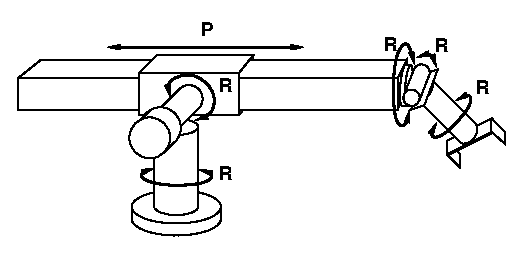
\includegraphics[width=0.5\linewidth]{figs/stanford-arm.eps}
	\end{center}
	\begin{itemize}
		\item 6 is the minimum number required to position end-effector arbitrarily
		\item For dynamical systems, add velocity for each DOF
		\item \textbf{Terminal effector} (or end effector): Tool usually attached to a robotic arm
	\end{itemize}
\end{frame}

\subsection{Manipulation}
\begin{frame}{Effectors}{Manipulation (II)}
	\vspace{-1cm}
   \begin{columns}
 	   \column{.60\textwidth}
			Big issue: Motion planning
			\begin{itemize}
				\item \textbf{Kinematics}: Given the pose, get the location
				\item \textbf{Inverse Kinematics}: Given the location, get the pose
			\end{itemize}
 	   \column{.40\textwidth}
	   		\begin{center}
			\begin{tikzpicture}
    \robotbase
	\angann{\thetaone}{$\theta_1$}
	\lineann[0.7]{\thetaone}{\Lone}{$L_1$}
	\link(\thetaone:\Lone);
	\joint
	\begin{scope}[shift=(\thetaone:\Lone), rotate=\thetaone]
	     \angann{\thetatwo}{$\theta_2$}
	     \lineann[-1.5]{\thetatwo}{\Ltwo}{$L_2$}
	     \link(\thetatwo:\Ltwo);
	     \joint
	     \begin{scope}[shift=(\thetatwo:\Ltwo), rotate=\thetatwo]
	           \angann{\thetathree}{$\theta_3$}
	           \lineann[0.7]{\thetathree}{\Lthree}{$L_3$}
	           \draw [dashed, red,rotate=\thetathree] (0,0) -- (1.2\ddx,0pt);
	           \link(\thetathree:\Lthree);
	           \joint
	           \begin{scope}[shift=(\thetathree:\Lthree), rotate=\thetathree]
	               \grip
	           \end{scope}
	     \end{scope}
    \end{scope}
\end{tikzpicture}
%\\
			\vspace{-0.2cm}
			\tiny{\href{http://www.texample.net/tikz/examples/three-link-annotated/}{(Source)}}
			\end{center}
	\end{columns}
\end{frame}

\subsection{Locomotion}
\begin{frame}{Effectors}{Locomotion (I)}
	\begin{center}
	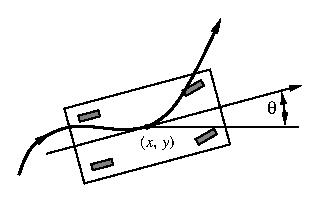
\includegraphics[width=0.4\linewidth]{figs/car-like.eps}
	\end{center}
	Two types of mobile robots
	\begin{itemize}
		\item \textbf{Holonomic}: Same DOF that control
		\item \textbf{Non-holonomic}: More DOF than controls
	\end{itemize}
	Control hardness depends on relation between DOF and control
	\begin{itemize}
		\item The larger is the gap, the harder is the control
		%\item Higher cost of holomic robots
	\end{itemize}
\end{frame}

\begin{frame}{Effectors}{Locomotion (II)}
	\centering Types of locomotion
	\bigskip	
	\begin{columns}
 	   \column{.25\textwidth}
		\centering 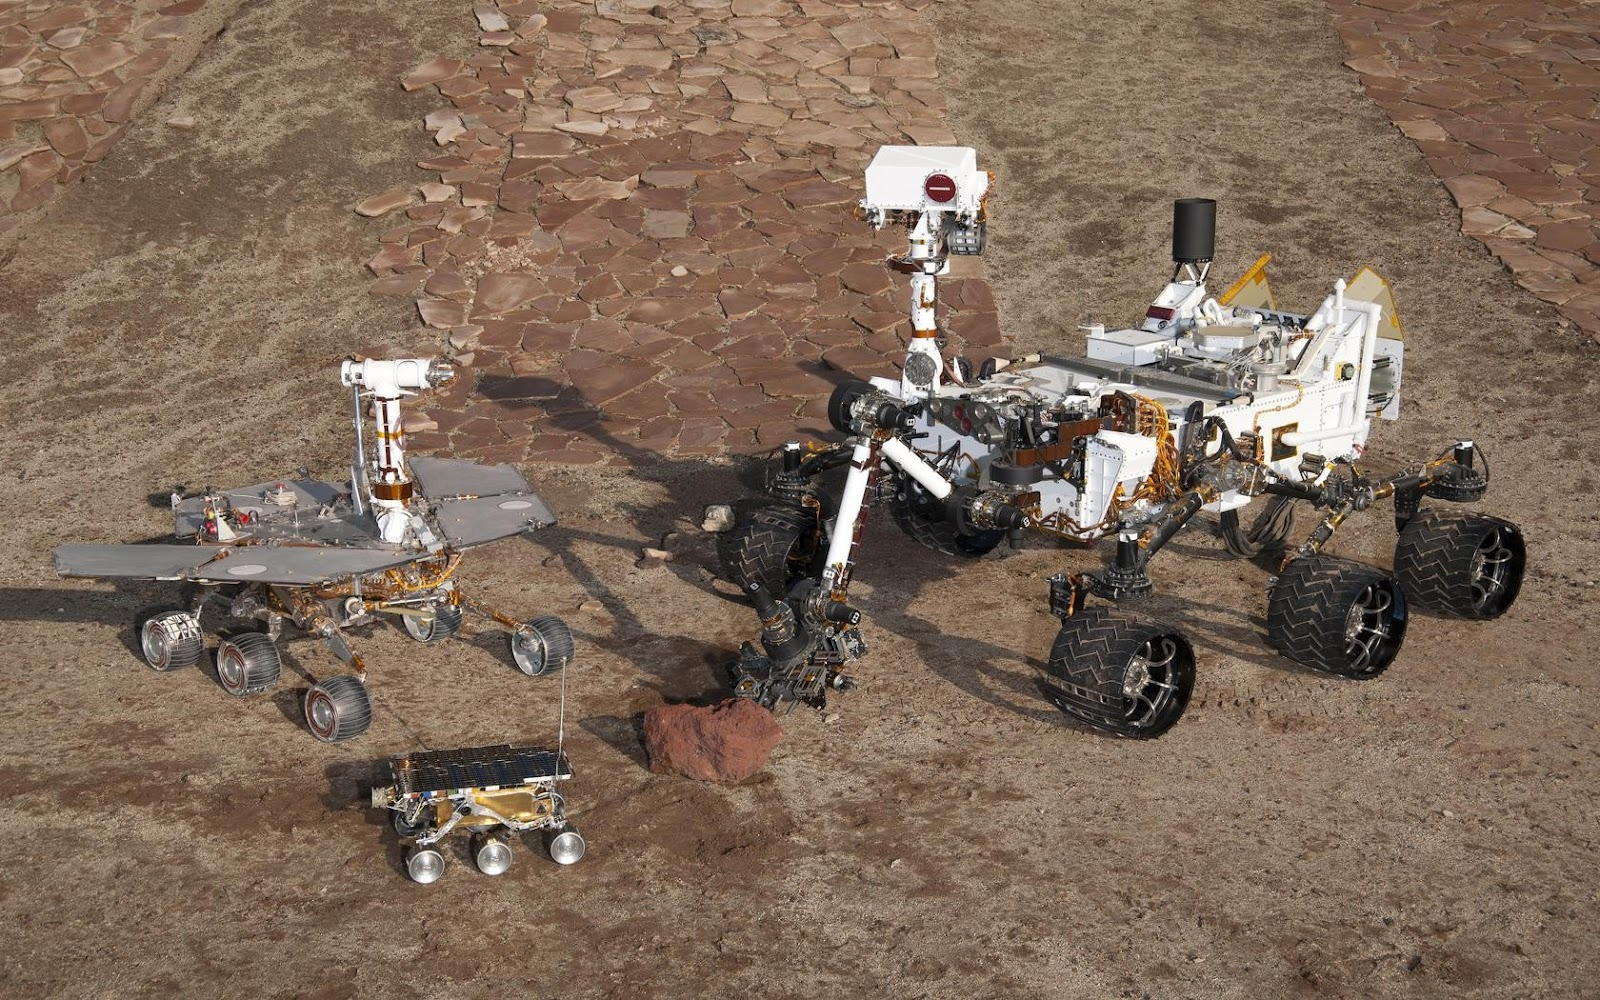
\includegraphics[width=\linewidth]{figs/curiosity.jpeg}\\\bigskip
		\centering 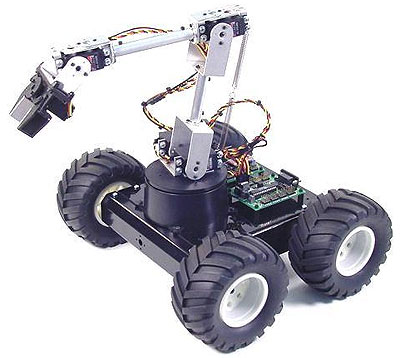
\includegraphics[width=\linewidth]{figs/rover.jpg}\\Rover
 	   \column{.25\textwidth}
		\centering 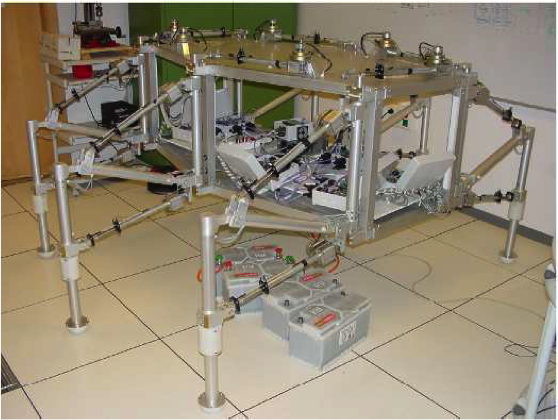
\includegraphics[width=\linewidth]{figs/ptinto.png}\\
		\centering 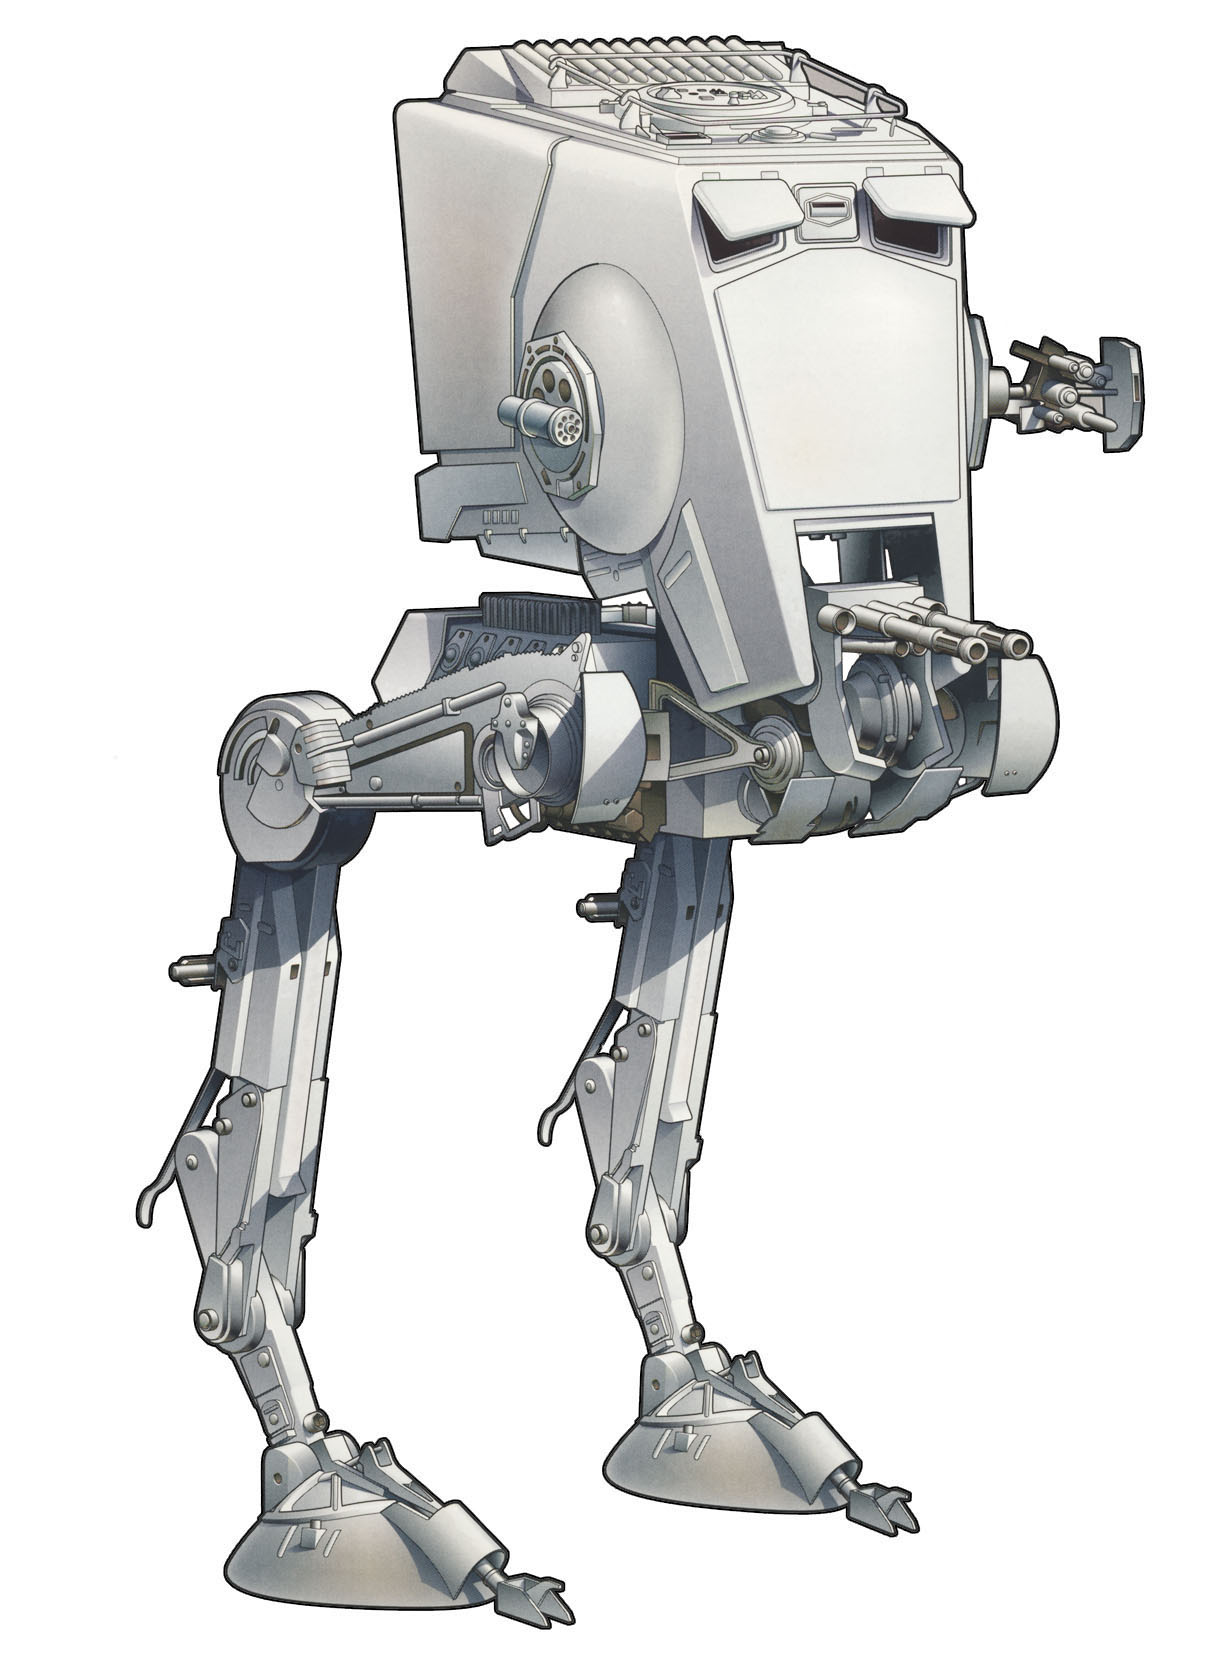
\includegraphics[width=0.9\linewidth]{figs/at-st.jpg}\\Walker
 	   \column{.25\textwidth}
		\centering 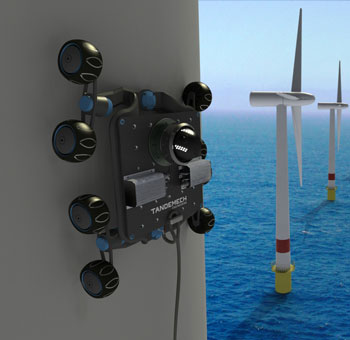
\includegraphics[width=\linewidth]{figs/climber.jpg}\\Climber
 	   \column{.25\textwidth}
		\centering 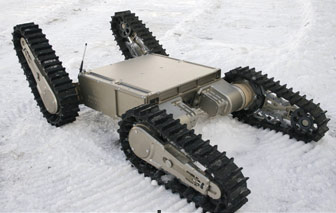
\includegraphics[width=\linewidth]{figs/tracks.jpg}\\Tracks
		\end{columns}
\end{frame}

\section{Sensors}

\subsection{Classification}
\begin{frame}{Sensors}{Classification}
	\textbf{Sensor}: Device that gathers information\\
	By energy emission:
	\begin{itemize}
		\item Passive
		\item Active
	\end{itemize}
	By function:
	\begin{itemize}
		\item Range sensors: Sonar, laser scanners, radar, tactile (like bumpers), ...
		\item Imaging sensors: Cameras (visual or infrared)
		\item Proprioceptive sensors: Encoders, inertial sensors, force sensors, torque sensors
	\end{itemize}
\end{frame}

\subsection{Range sensors}
\begin{frame}{Sensors}{Range sensors: Sonar}
	Provides a single distance measure
	\begin{itemize}
		\item Uses a sound pulse, usually ultrasound
		\item Short distance, usually for obstacle detection
		\item Not very precise
		\item Cheap ($\pm$ 2.5 euro)
	\end{itemize}
	\begin{center}
	\begin{columns}
 	   \column{.15\textwidth}
 	   \column{.25\textwidth}
	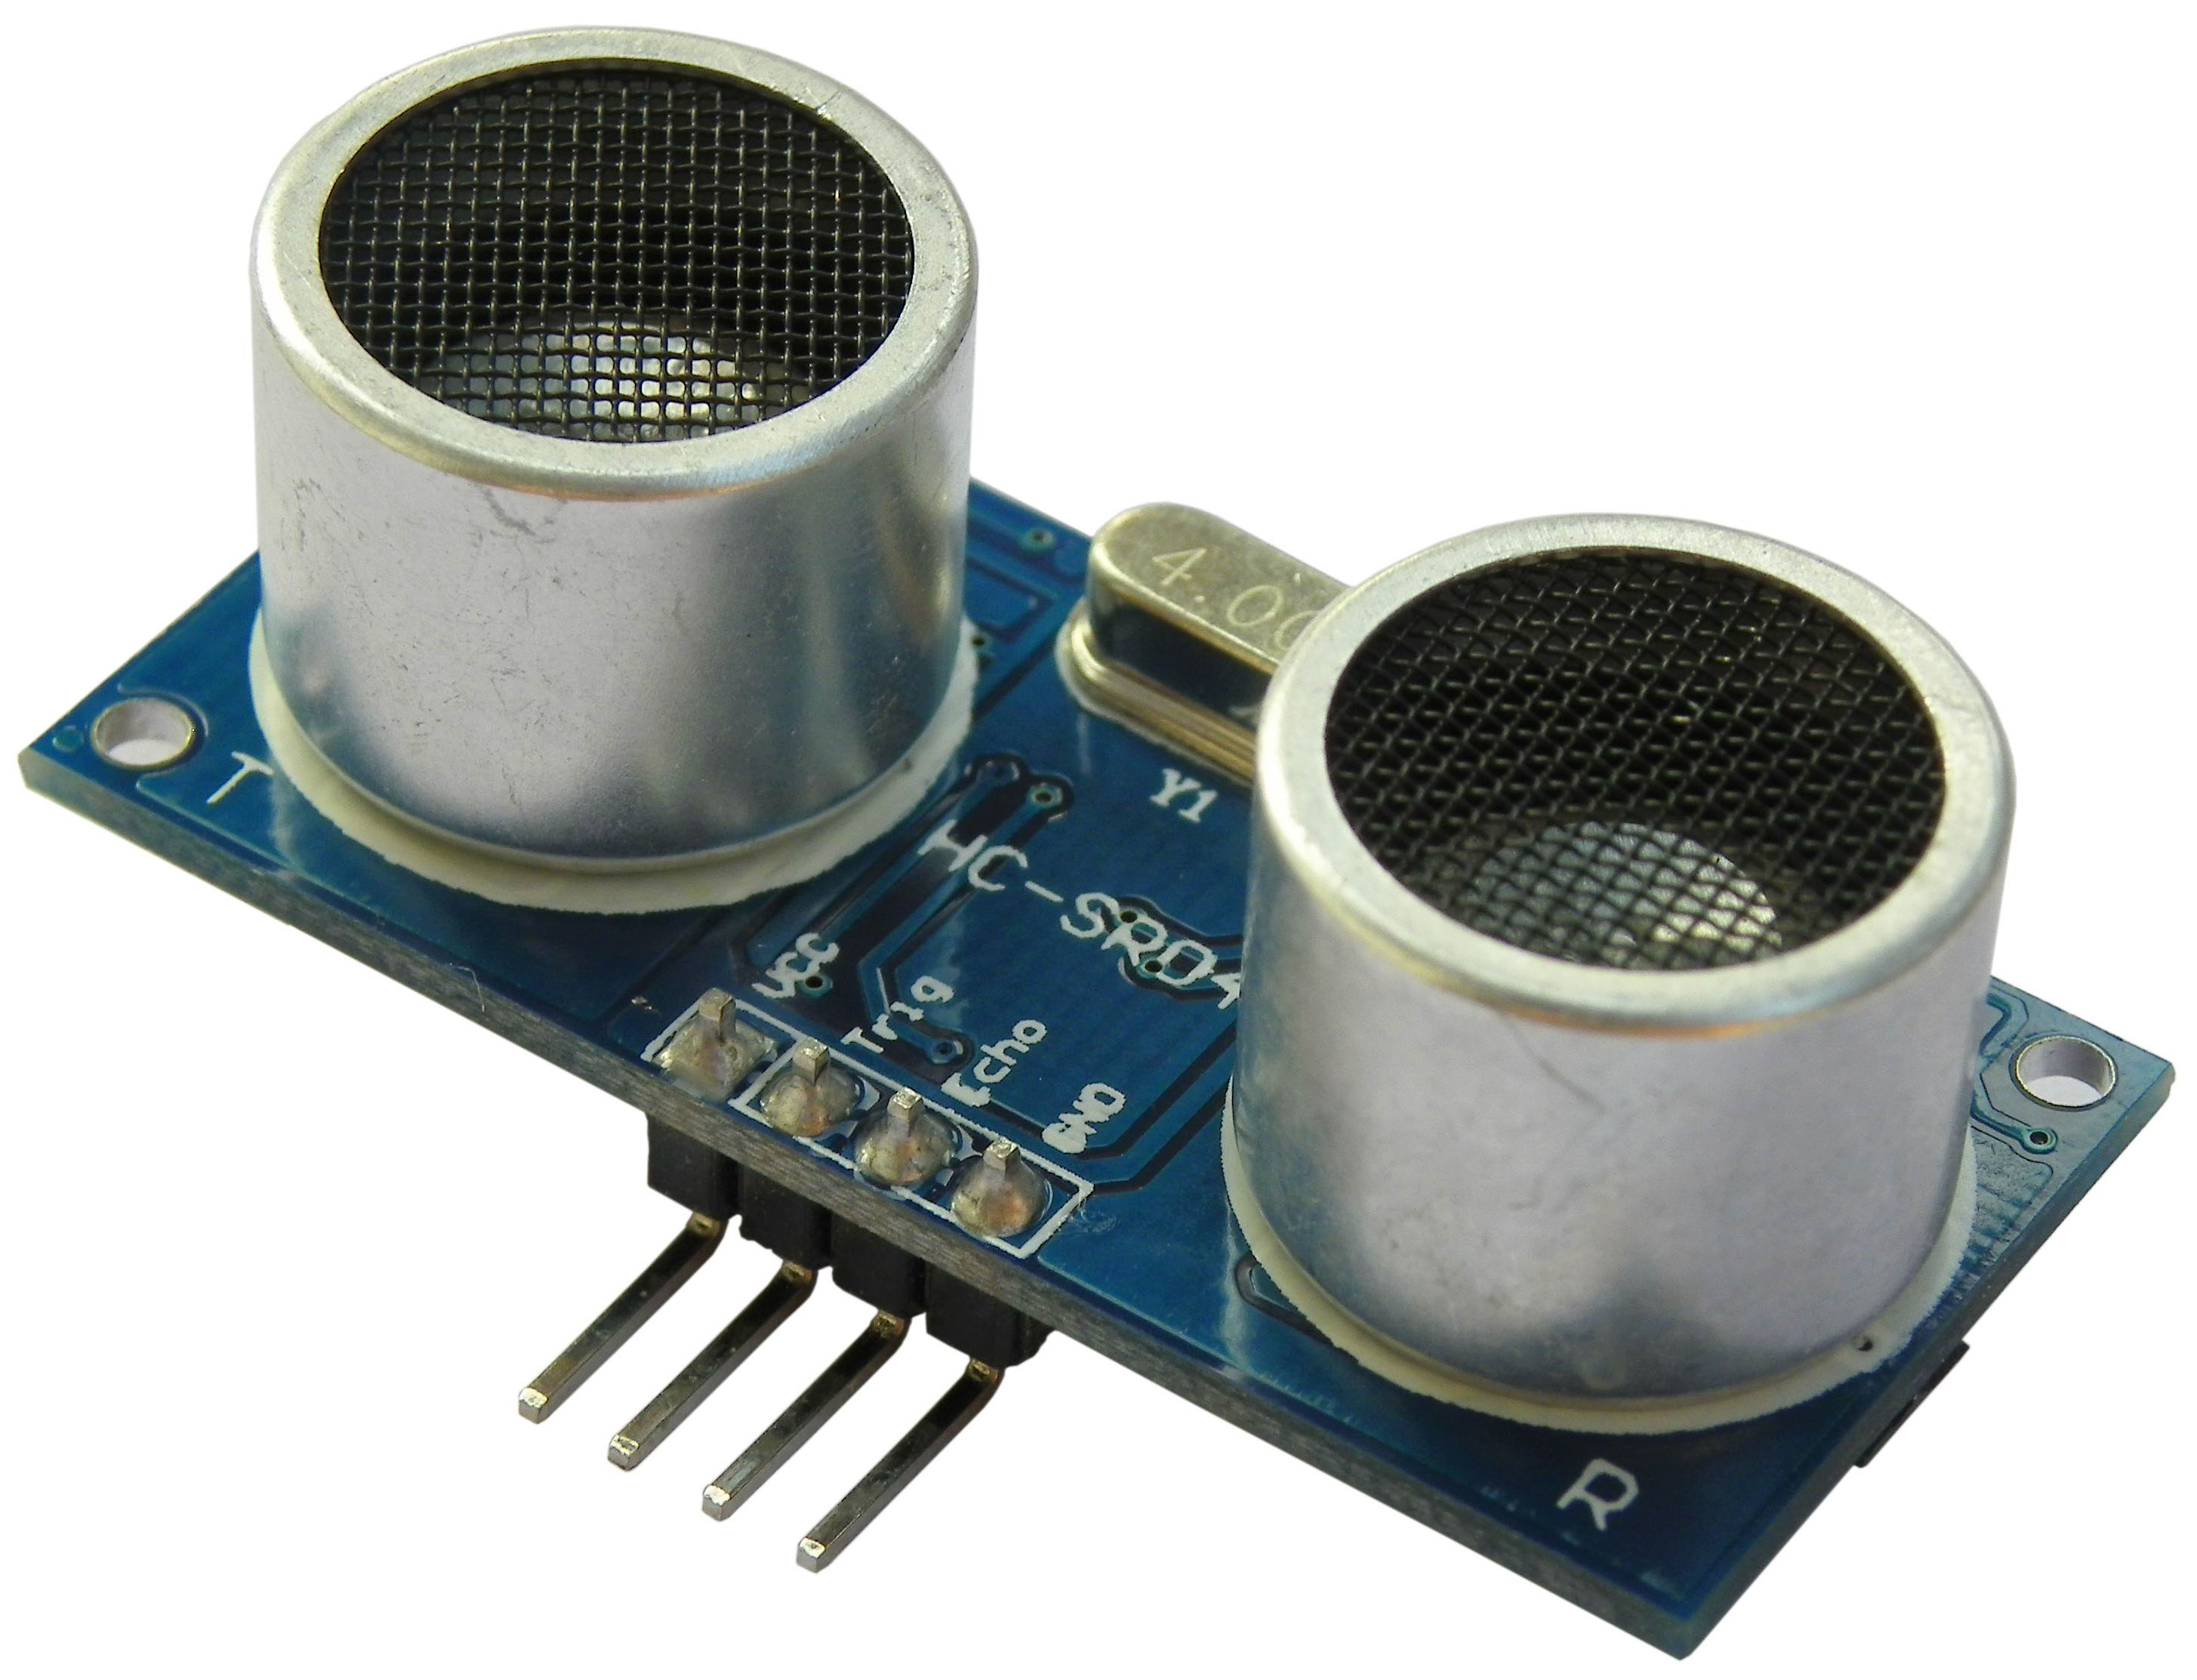
\includegraphics[width=\linewidth]{figs/ultrasound.jpg}
 	   \column{.02\textwidth}
 	   \column{.25\textwidth}
	\includegraphics[width=\linewidth]{figs/lares.jpg}
 	   \column{.02\textwidth}
 	   \column{.25\textwidth}
	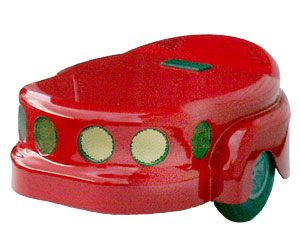
\includegraphics[width=\linewidth]{figs/amigobot.jpg}
 	   \column{.15\textwidth}
	\end{columns}
	\end{center}
\end{frame}

\begin{frame}{Sensors}{Range sensors: Laser scanners}
	Provides precise ranges
	\begin{itemize}
		\item Several laser beams
		\item Extremely precise
		\item 1D, 2D and 3D laser scanners
		\item Very expensive (thousands)
		\item Useful for SLAM
	\end{itemize}

	\begin{center}
	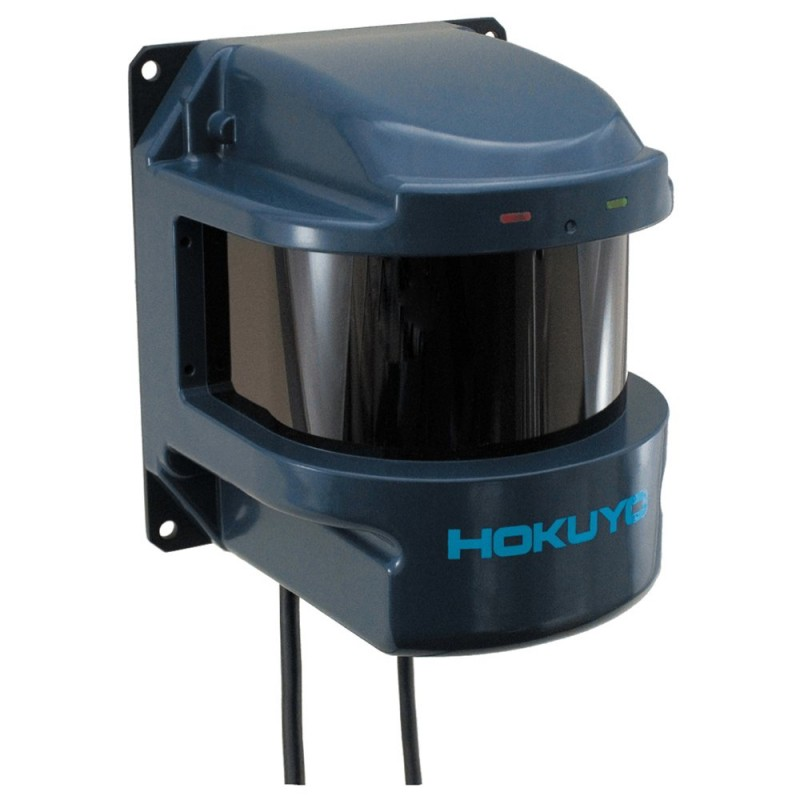
\includegraphics[width=0.2\linewidth]{figs/laser.jpg}\quad
	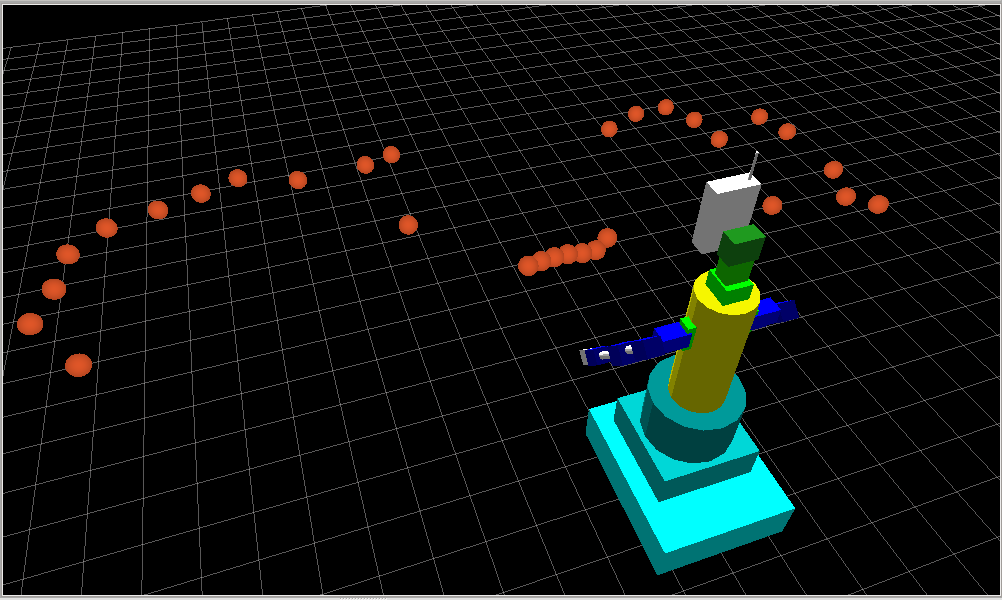
\includegraphics[width=0.4\linewidth]{figs/laserscan.png}
	\end{center}
\end{frame}

\subsection{Imaging sensors}
\begin{frame}{Sensors}{Imaging sensors: Cameras}
	Provides images of the environment
	\begin{itemize}
		\item Different wavelengths (visible or infrared)
		\item Very important in Robotics
		\item With proper algorithms, it is almost an universal sensor
		\item Need of \alert{computer vision}
			\begin{itemize}
			\item Object recognition, face recognition, obstacle detection, etc
			\end{itemize}
		\item From cheap to expensive
	\end{itemize}

	\begin{center}
	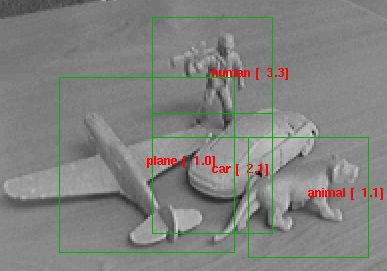
\includegraphics[width=0.3\linewidth]{figs/computervision.png}\enspace
	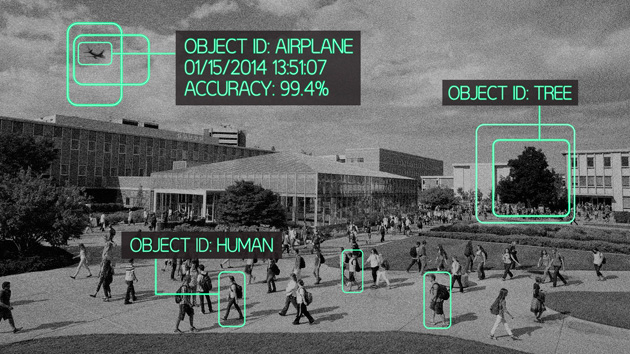
\includegraphics[width=0.33\linewidth]{figs/computervision2.jpg}\enspace
	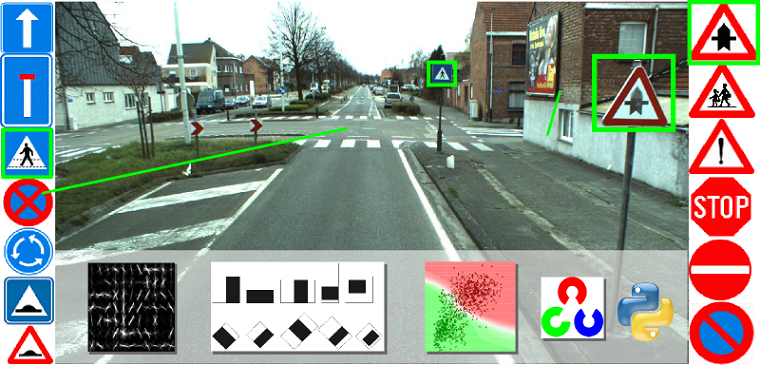
\includegraphics[width=0.33\linewidth]{figs/computervision3.png}
	\end{center}
\end{frame}

\begin{frame}{Sensors}{Imaging sensors: Stereovision}
	Two parallel cameras
	\begin{itemize}
		\item Information fusion provides depth
		\item Similar to human vision
		\item The ``poor man'' alternative to laser scans
		\item Quite popular in Robotics
	\end{itemize}

	\begin{center}
	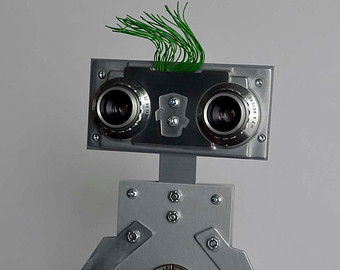
\includegraphics[width=0.3\linewidth]{figs/stereo.jpg}\enspace
	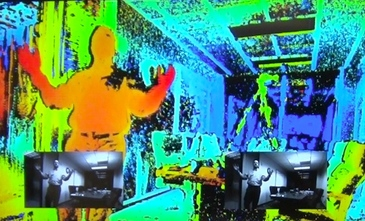
\includegraphics[width=0.3\linewidth]{figs/stereovision.jpg}\enspace
	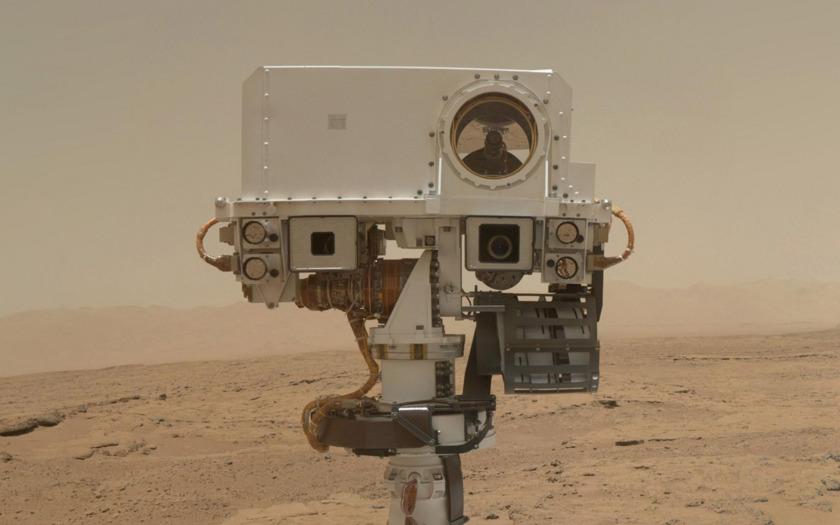
\includegraphics[width=0.3\linewidth]{figs/curiositystereo.jpg}
	\end{center}
\end{frame}

\begin{frame}{Sensors}{Imaging sensors: Depth sensors}
	Provides image and depth 
	\begin{itemize}
		\item Active depth sensor
		\item Kinect-type sensors
		\item Increasing popularity in Robotics
	\end{itemize}

	\begin{center}
	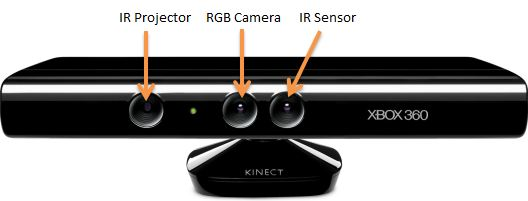
\includegraphics[width=0.3\linewidth]{figs/kinect.JPG}\enspace 
	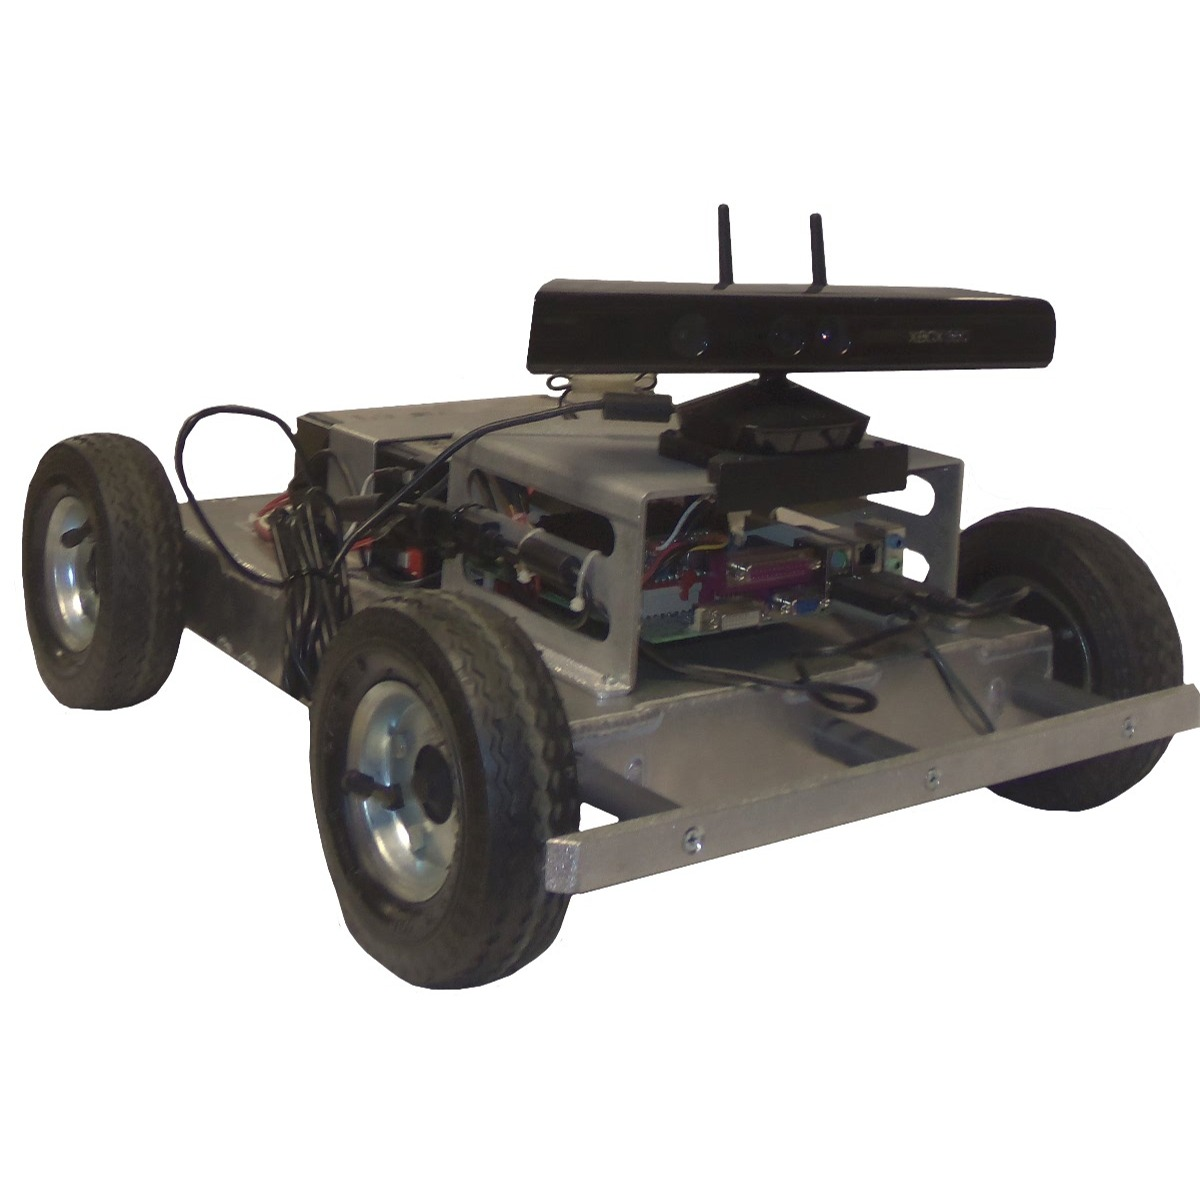
\includegraphics[width=0.3\linewidth]{figs/kinectrobot.jpg}\enspace 
	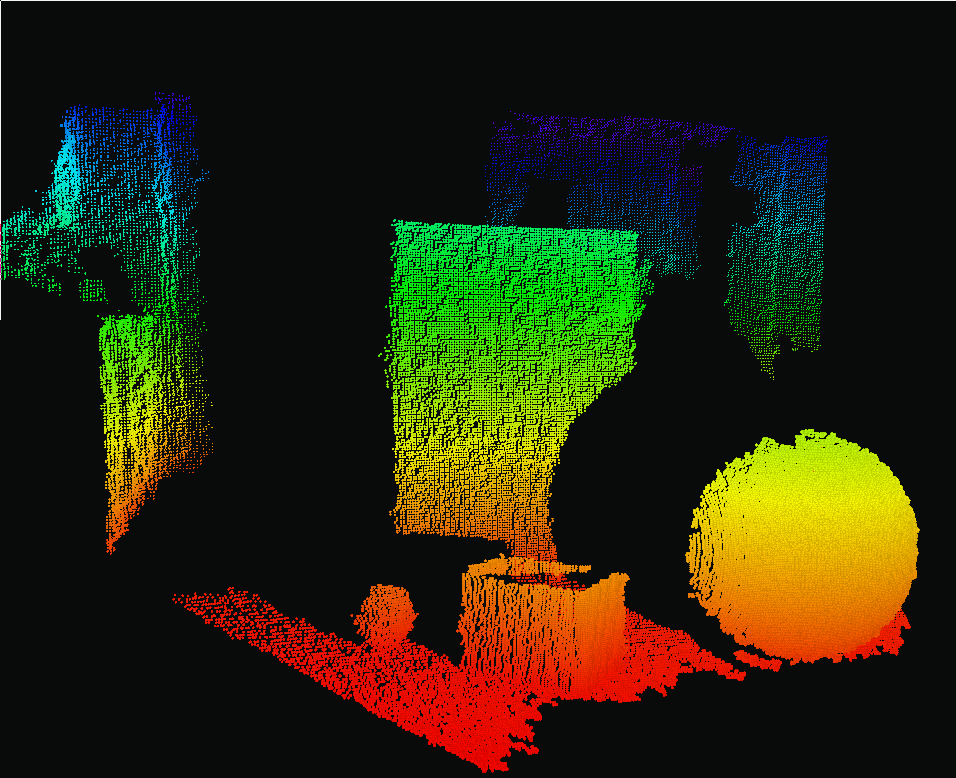
\includegraphics[width=0.3\linewidth]{figs/kinectrviz.png}
	\end{center}
\end{frame}

\subsection{Proprioceptive sensors}

\begin{frame}{Sensors}{Proprioceptive sensors}
	Sensors that provide information about the robot state
	\begin{itemize}
		\item Encoders, inertial sensors, force sensors, torque sensors, ...
		\item Needed for \alert{odometry}
	\end{itemize}
	\textbf{Odometry}: Estimate of change in position over time
	\begin{itemize}
		\item Theoretical position differs from actual position
		\item Unbalanced motors, power unstability, sliding wheels, ...
	\end{itemize}
	\begin{center}
	
\includegraphics[width=0.2\linewidth]{figs/encoder.png}\quad
	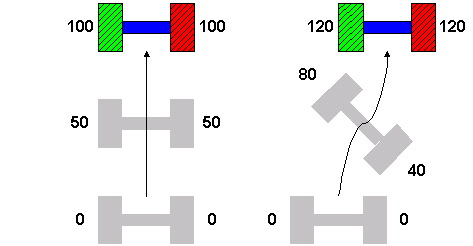
\includegraphics[width=0.4\linewidth]{figs/odometry.jpg}
	\end{center}
\end{frame}

\section{Robotic perception}
\subsection{Perception}
\begin{frame}{Navigation}{Perception}
	Mobile robots move around a physical environment
	\begin{itemize}
		\item Perception: Transform \textit{noisy} sensor data into environment models
	\end{itemize}
	Perception must satisfy three conditions
	\begin{itemize}
		\item Complete 
		\item Structured
		\item Reliable
	\end{itemize}
	Three problems
	\begin{itemize}
		\item Localization (unknown location)
		\item Mapping (unknown map)
		\item SLAM (unknown location and map)
	\end{itemize}
\end{frame}

\subsection{Localization}
\begin{frame}{Navigation}{Localization}
	\begin{columns}
 	   \column{.65\textwidth}
	\textbf{Localization}: Where is the robot within the world?
	\begin{itemize}
		\item Unknown location, known map
		\item Problem: Relate sensor readings to the world
	\end{itemize}
	Three problems
	\begin{itemize}
		\item Tracking, initial position known
		\item Global localization, initial position unknown
		\item Re-localization, incorrect known position (\alert{kidnapped robot} problem)
	\end{itemize}
	Beacons: RFID tags, visual marks, QR codes, etc
 	   \column{.35\textwidth}
		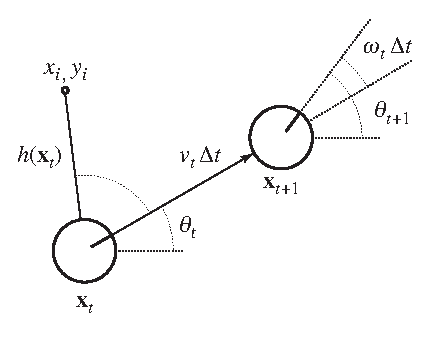
\includegraphics[width=0.9\linewidth]{figs/robotics-pic2.eps}\\
		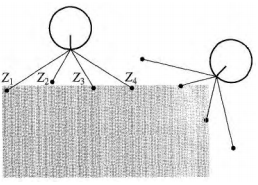
\includegraphics[width=0.9\linewidth]{figs/sensors-nav.png}
	 \end{columns}
\end{frame}

\begin{frame}{Navigation}{Localization: Monte-Carlo Localization (I)}
	Monte-Carlo Localization (MCL)
	\begin{itemize}
		\item A type of particle filter
		\item Estimates robot location and orientation
		\item Uses a distribution of random particles that converge to robot position
		\item Prediction of sensor values after motion and compares with measures
	\end{itemize}	
	\href{https://www.youtube.com/watch?v=aUkBa1zMKv4}{(Video particle filter)}\\
	\href{https://www.youtube.com/watch?v=lCXv4yOcwf8}{(Video)}
\end{frame}

\begin{frame}{Navigation}{Localization: Monte-Carlo localization (II)}
	\begin{center}
	 	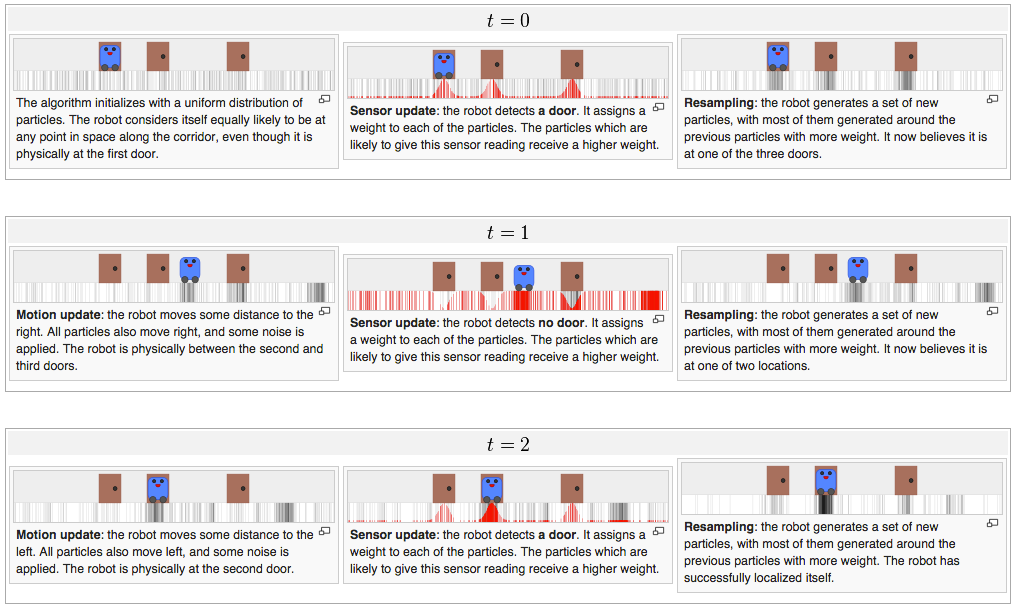
\includegraphics[width=\linewidth]{figs/montecarlo.png}\\
		\tiny{\href{https://en.wikipedia.org/wiki/Monte_Carlo_localization}{(Source)}}
	\end{center}
\end{frame}

\begin{frame}{Navigation}{Localization (III): Kalman filters}
	Kalman filters (or Extended Kalman Filters, EKF)
	\begin{itemize}
		\item Extended Kalman Filters, or EKF, is a popular extension
		\item Based on Bayesian Statistics
		\item Optimal for linear systems with Gaussian noise
			\begin{itemize}
			\item Otherwise, MCL outperforms EKF
			\item Needs less computational resources than MCL
			\end{itemize}
		\item EKF used for normal operation, MCL used to solve ambigueties
	\end{itemize}
	\bigskip
	\begin{center} 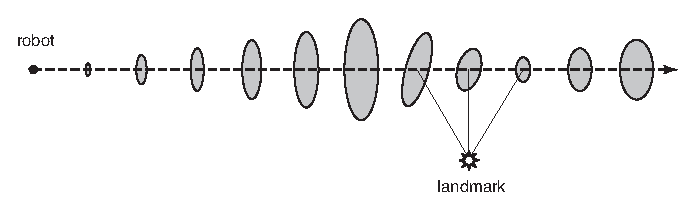
\includegraphics[width=0.7\linewidth]{figs/robotics-pic6.eps}
	\end{center}
\end{frame}

\subsection{Mapping}

\begin{frame}{Navigation}{Mapping}
	\textbf{Mapping}: How is the wold around the robot?
	\begin{itemize}
		\item Known location, unknown map
		\item Build map
	\end{itemize}
	Problem: Integrate sensor measurements to produce a map\\
	\href{https://www.youtube.com/watch?v=8HdgliagAds}{(Video Underground Mine Mapping)}
\end{frame}

\begin{frame}{Navigation}{Mapping: Map models}
	\begin{center}
	\begin{columns}
 	   \column{.1\textwidth}
 	   \column{.32\textwidth}
	   	\begin{center}Grid-based\\\bigskip
		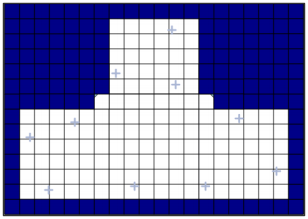
\includegraphics[width=\linewidth]{figs/grid.png}\\
		\end{center}
		Collection of discretized pixels
 	   \column{.02\textwidth}
 	   \column{.32\textwidth}
	   	\begin{center}Feature-based\\\bigskip
		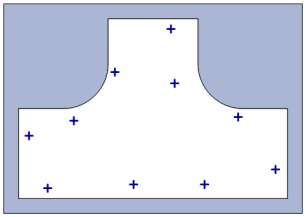
\includegraphics[width=\linewidth]{figs/feature.png}\\
		\end{center}
		Collection of landmark locations
 	   \column{.02\textwidth}
 	   \column{.32\textwidth}
	   	\begin{center}Topological-based\\\bigskip
		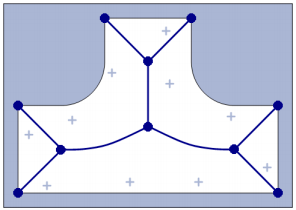
\includegraphics[width=\linewidth]{figs/topological.png}\\
		\end{center}
		Collection of nodes and links
 	   \column{.1\textwidth}
	\end{columns}
	\bigskip
	\tiny{\href{http://www.cs.cmu.edu/~motionplanning/lecture/Chap8-Kalman-Mapping_howie.pdf}{(Source)}}
	\end{center}
\end{frame}

\begin{frame}{Navigation}{Mapping: Voronoi map}
	Voronoi diagram: Partition of a plane into regions based on distance points
	\begin{itemize}
	   \item Regions boundaries maximize distance to obstacles
	   \item Mapping of boundaries into graphs
	\end{itemize}

	\begin{columns}
 	   \column{.15\textwidth}
 	   \column{.35\textwidth}
			\centering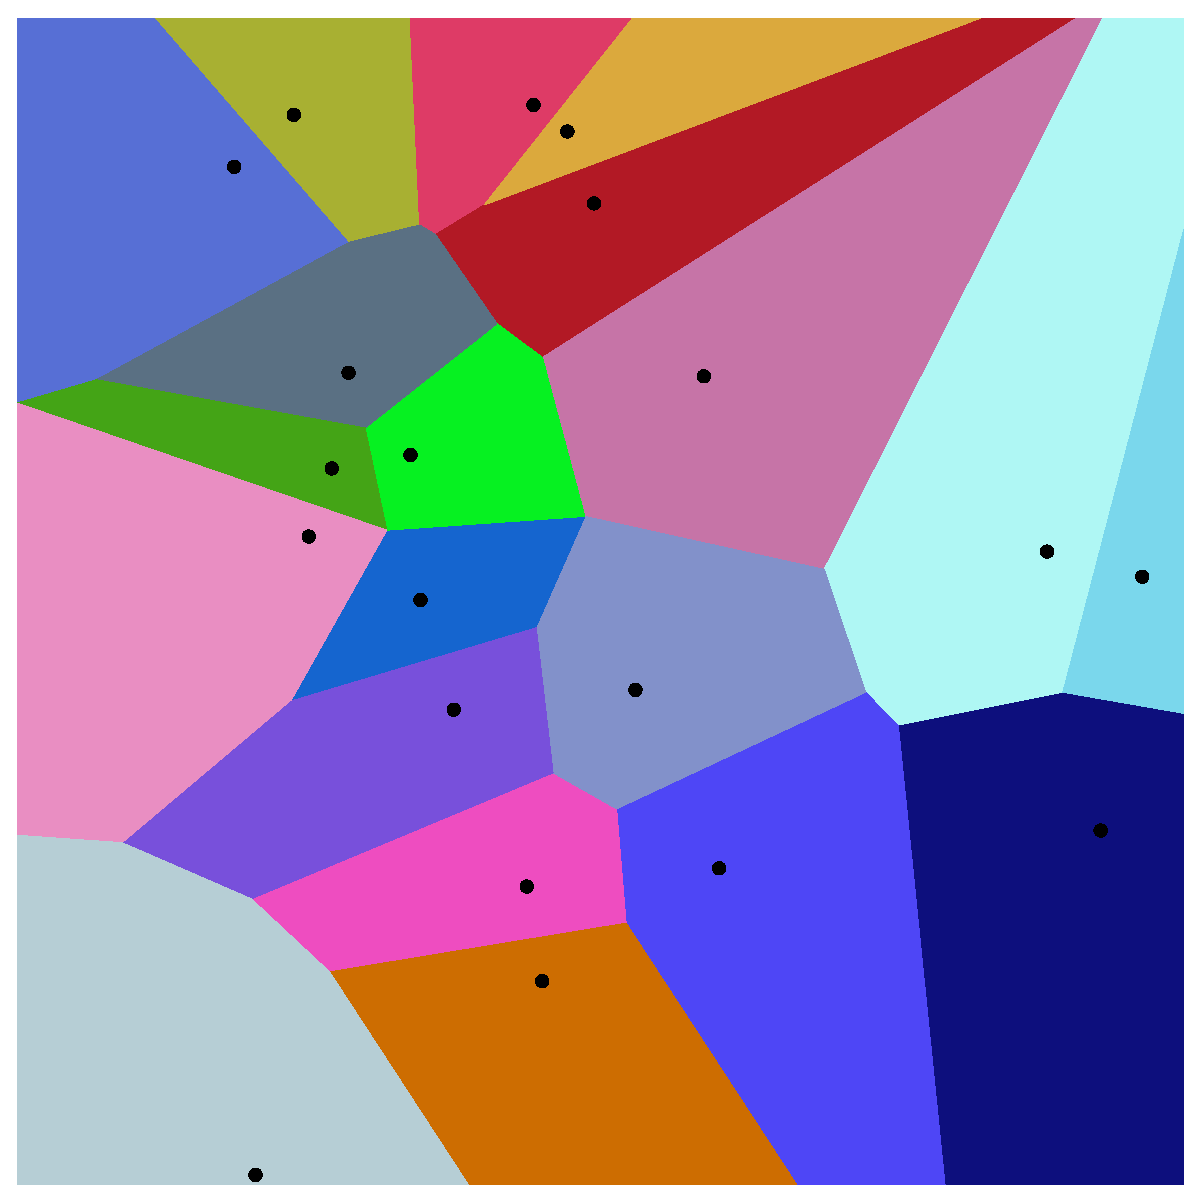
\includegraphics[width=\linewidth]{figs/voronoi.eps}
 	   \column{.35\textwidth}
			\centering
\includegraphics[width=\linewidth]{figs/armVoronoi.eps}
 	   \column{.15\textwidth}
	\end{columns}

	\begin{center}
		\tiny{\href{https://upload.wikimedia.org/wikipedia/commons/5/54/Euclidean_Voronoi_diagram.svg}{(Source)}}
	\end{center}
\end{frame}

\subsection{SLAM (Simultaneous Localization and Mapping)}

\begin{frame}{Navigation}{SLAM}
	\begin{columns}
 	   \column{.65\textwidth}
		SLAM: Map and location are unknown
		\begin{itemize}
			\item Big, big problem in Robotics
			\item Huge number of applications
		\end{itemize}
		SLAM techniques
		\begin{itemize}
			\item Extended Kalman filters (EKF)
			\item Occupancy Grid Mapping
		\end{itemize}

 	   \column{.35\textwidth}
			\centering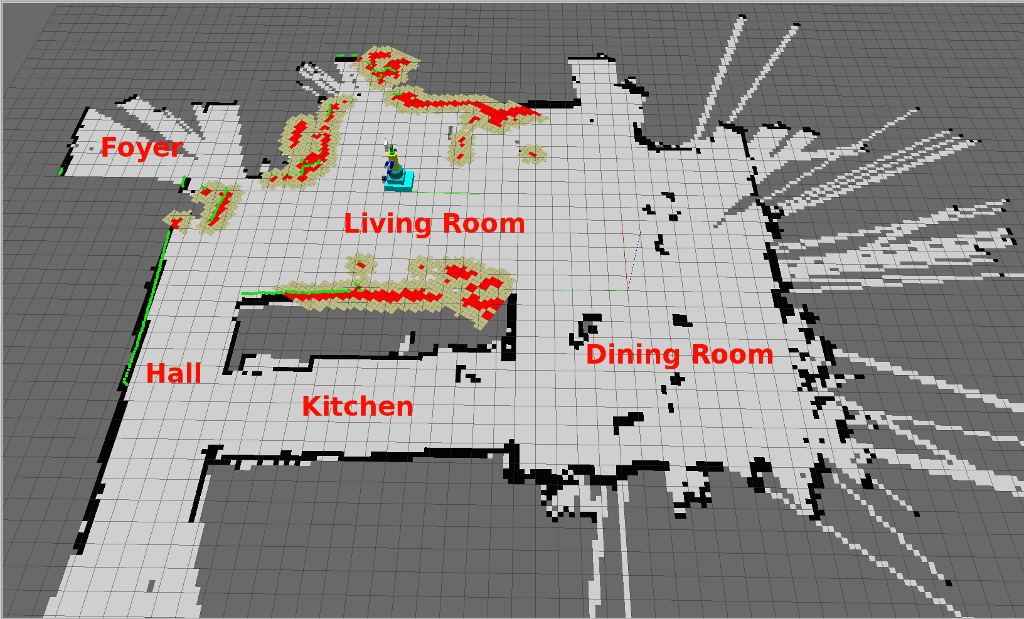
\includegraphics[width=\linewidth]{figs/slam2d.png}\\
			\tiny{\href{https://www.youtube.com/watch?v=17W8dkzkvWA}{(Video SLAM)}}
			\bigskip
			\centering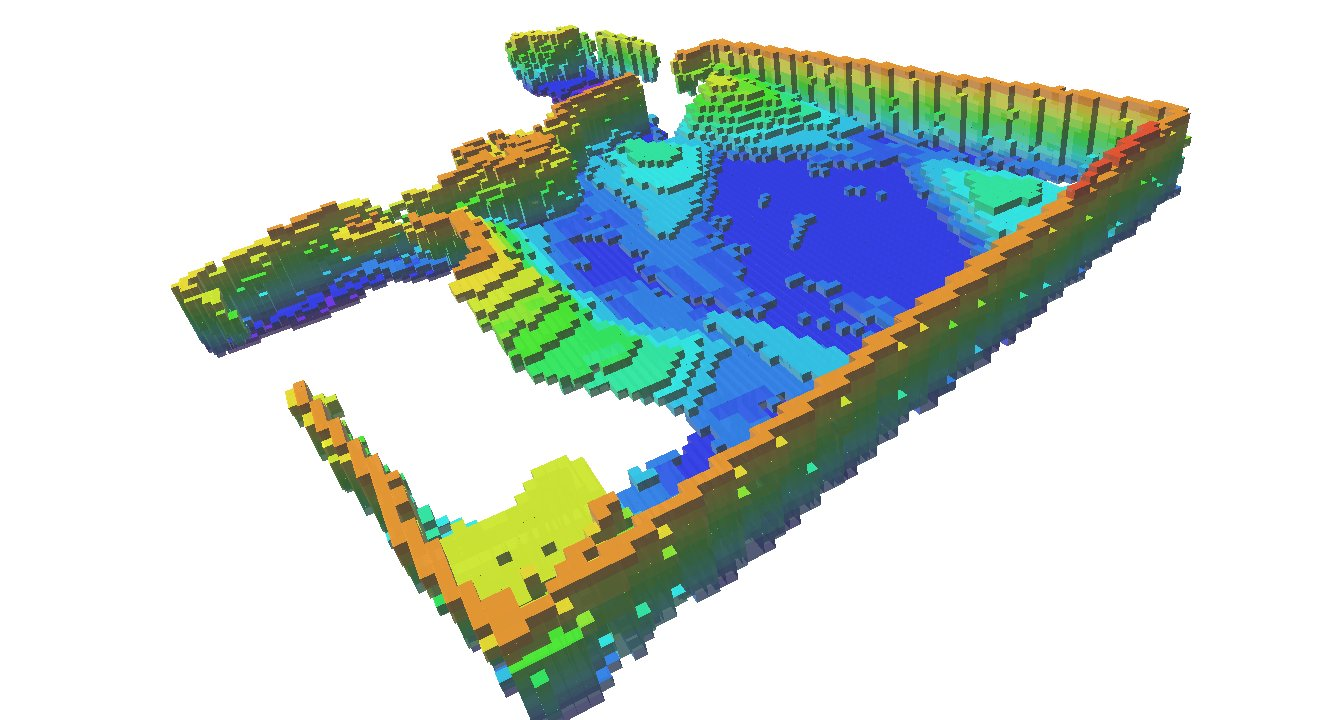
\includegraphics[width=\linewidth]{figs/slam3d.jpg}\\
			\tiny{\href{https://www.youtube.com/watch?v=qpTS7kg9J3A}{(Video 3D SLAM)}}
	\end{columns}

\end{frame}


\end{document}
